\documentclass[a4paper,listof=leveldown,listof=numbered]{scrreprt}

\usepackage[ngerman]{babel}
\usepackage[utf8]{inputenc}
\usepackage[T1]{fontenc}
\usepackage{todonotes}
\usepackage{ae}
\usepackage{float}
\usepackage{booktabs}
\usepackage{multirow}
\usepackage{colortbl}
\usepackage{tabularx}
\usepackage[printonlyused]{acronym}
\usepackage[automark,headsepline,ilines,komastyle, plainfootsepline]{scrpage2} 
\usepackage[bookmarks,bookmarksnumbered]{hyperref}

\newcommand{\gray}{\rowcolor[gray]{.90}}
\newcolumntype{C}{>{\Centering}X} %Tabularx zentrieren

%Kopf- und Fußzeile---------------------------
\pagestyle{scrheadings}
\clearscrheadings
\lohead{\headmark}
\rohead{Software-Engineering Gruppenarbeit}
\lofoot[Gmeiner, Rezmer, Zeiler]{Gmeiner, Rezmer, Zeiler}
\cofoot{\pagemark}
\rofoot[\today]{\today}
\cfoot{\pagemark}
\setheadsepline{.4pt} % Linie unter dem Head
\setfootsepline{.4pt} % Ganzunten
%---------------------------------------------

\begin{document}
% Titelseite	
	\begin{titlepage}

\begin{center}


% Oberer Teil der Titelseite: Firmenlogo/Projektlogo
%\includegraphics[width=0.15\textwidth]{./logo}\\[1cm]    

\textsc{\LARGE TINF13IN GmbH}\\[2cm]

\textsc{\Large Pflichtenheft für}\\[1 cm]


% Title
\newcommand{\HRule}{\rule{\linewidth}{0.5mm}}
\HRule \\[0.4cm]
{\fontsize{60}{65} \bfseries \selectfont ScOREO}\\ [0.4cm]

\HRule \\[2.5cm]

% Author and supervisor
\begin{minipage}{0.4\textwidth}
\begin{flushleft} 
\end{flushleft}
\end{minipage}
\hfill
\begin{minipage}{0.4\textwidth}
\begin{flushright} \large
\emph{erstellt von:} \\
Alexander \textsc{Rezmer}\\
Fabian \textsc{Zeiler}\\
Christian \textsc{Gmeiner}
\end{flushright}
\end{minipage}

\vfill

% Unterer Teil der Seite
\large
{\large \today\\
\emph{Version:} v0.9}

\end{center}

\end{titlepage}
	
% Römische Nummerierung	
	\pagenumbering{Roman}
	
% Platzierung des Inhaltsverzeichnisses
	\tableofcontents

% Zielbestimmung
	\chapter{Zielbestimmung}
\pagenumbering{arabic}
	Das im Folgenden beschriebene Programm soll die Grundlage für ein Bewertungssystem für Prüfer sein. Mit diesem System soll eine gerechte und einfache Bewertung ermöglicht werden. Dies wird sichergestellt indem die einzelnen Bewertungen auf einen gemeinsamen Score umgerechnet werden. Zusätzlich ist dieses System so aufgebaut, dass es sich sehr leicht an neuen Prüfungsbedingungen anpassen lässt. Durch verschiedene Gewichtungen der Scores ergibt sich die Möglichkeit einzelne Bewertungen stärker zu werten als andere. Eine weitere Funktionalität des Programmes soll es dem Prüfer ermöglichen zum Score ebenfalls eine Rückmeldung anzuhängen um dem Prüfling ein Feedback zu geben. Genau so soll der Prüfling (ggf. Student) ein Feedback anfordern können um eine Begründung zu für seine Bewertung erhalten zu können.
	
	\section{Musskriterien}
	Die Software muss eine korrekte Umrechnung der Bewertungen in gültige Scores beherrschen, welche die Prüfer eintragen. Da es sich bei diesen um teilweise sensible Daten handelt, müssen diese gut geschützt sein, sodass sie von außerhalb nicht verändert werden können. Dieses Programm bietet die Möglichkeit durch ein zweistufiges holistisches Bewertungssystem die Bewertungen einzutragen. Bei diesem zweistufigen System kann der Prüfer die Stufen selbst so gewichten wie er es für sinnvoll hält. Mehrere Bewertungen können miteinander verrechnet und einzeln gewichtet werden. Am Ende soll der Prüfer ein Score bekommen, welcher sich aus seinen Bewertungen und Gewichtungen errechnen lässt. Die Software muss auf Windows PCs lauffähig sein, da dies die am meisten verwendete Laufzeitumgebung ist. Des weiteren muss das System einfach zu bedienen sein. Der Prüfer muss die Ergebnis seiner Bewertung einfach an die Studenten weiter geben können. Dies kann durch einen Ausdruck dieser statt finden wie auch durch ein eigenes Programm welches den Studenten Zugriff auf die jeweiligen Scores liefert. Umrechnung von der Inversen muss auch voll funktionsfähig sein. 
	
	\section{Wunschkriterien}
	Das Grundprogramm soll wie ein Gerüst dienen, sodass man verschiedene \ac{Add-On} einbinden kann. Dieses Zusatzapplikationen können weitere Bewertungsmöglichkeiten beziehungsweise Umrechnungen zwischen diesen Bewertungen sein. Es kann sich dabei auch um eine Anbindung an bestehende Systeme verschiedener anderer Anbieter handeln. Später, wenn das Backend funktionsfähig ist, soll durch eine Website ein Zugriff ermöglicht werden um von Mobilen Endgeräte oder jedem anderen Gerät welches einen Browser besitzt darauf zugreifen zu können. Des weiteren soll eine \ac{API} implementiert werden, mit welcher andere Programme mit diesem Programm kommunizieren können. Es soll eine iOS App erstellt werden um bequem von iPad/iPhone darauf zugreifen zu können.
	
	\section{Abgrenzungskriterien}
	Das Produkt soll keine Software werden, mit welcher die Studenten untereinander verglichen werden. Dies kann gegebenen falls durch \acs{Add-On} ermöglicht werden, es gehört jedoch nicht zu diesem Projekt dazu. Des weiteren soll die Software kein Netzwerk darbieten in welchem unterschiedlichen Prüfer sich mit anderen austauschen können und die Prüfungsergebnisse untereinander vergleichen zu können.
	

% Produkteinsatz
	\chapter{Produkteinsatz}
	Der geplante Einsatz des Systems sind die Qualitätsanforderungen.
	
	\section{Anwendungsbereiche}
	Das System soll vor allem zur Bewertung von Schülern und Studenten dienen. Es können jedoch auch andere Institutionen oder Firmen, welche ein einheitliches Bewertungssystem wollen, welches eine faire Bewertung ermöglicht. Es muss jedoch garantiert werden, dass keine fremden Personen Zugriff auf das System bekommen, da es sich bei solchen Bewertungen um teils sensible Informationen handelt. Studenten sollten die einfache Möglichkeit besitzen nachdem sie einen Test durchlaufen haben ihre Bewertung zu erfahren und diese auf einer einfachen Oberfläche teils grafisch dargestellt werden soll um einen Vergleich zu ermöglichen.
	
	\section{Zielgruppen}
	\begin{itemize}
		\item \underline{Prüfer:}\\
	Der Prüfer ist der Ersteller sowie der Bearbeiter der Prüfung. Dieser muss sich sinnvolle Bewertungskriterien überlegen, sowie in das System eintragen. Der Prüfer benötigt alle Funktionen zum Eintragen der Bewertungen bzw. der Scores.
	
		\item \underline{Verwalter (Admin):}\\
	Der Verwalter besitzt die Rechte zur Erstellung sowie Löschung der Benutzer. Zusätzlich kann er Benutzergruppe erstellen sowie die Benutzer in die jeweiligen Benutzergruppen zuordnen. Entweder ist der Benutzer ein Student oder Dozent / Prüfer. Der Verwalter kann zusätzlich die Bewertungen verwalten.
			
		\item \underline{Verwaltung:}\\
	Die Verwaltung benötigt Zugriff auf das System um die Score auslesen zu können. Diese werden in einem Archiv abgespeichert und für 10 Jahre hinterlegt. 	
	
	\item \underline{Dozent:}\\
	Der Dozent besitzt die gleichen Rechte wie der Prüfer.
		
	\end{itemize}

	\section{Betriebsbedingungen}
	
	\begin{itemize}
	\item \underline{Physikalische Umgebung:}\\
	Die Software soll später auf jedem Computer lauffähig sein. Die Datenbank mit API wird auf einem Server installiert. Somit besteht die Möglichkeit, dass mehrere Personen gleichzeitig Zugriff auf die Daten haben. Über ein kleines Programm kann der Prüfer sich mit der Datenbank verbinden und darauf zuzugreifen.
	
	\item \underline{Tägliche Betriebszeit:} \\
	Der Server auf dem die Daten hinterlegt sind muss immer verfügbar sein, damit die Prüfer wie auch die Prüflinge jederzeit mit der Anwendung Zugriff haben.
	Ein reduziertes Programm (Prototyp) wird vor dem eigentlichen Programm entwickelt.
		
	\item \underline{Betrieb:} \\
	Es ist ein unbeaufsichtigter Betrieb vorgesehen. Sobald der Server einmal installiert ist, sollte das System ohne weitere Konfigurationen funktionieren. Der Prüfer sollte sich nicht mit der Konfiguration des System belasten müssten. 	
	\end{itemize}
	
	
% Produktübersicht
	\chapter{Produktübersicht}
	Im Folgenden auf Abb~\ref{fig:usecase} wird der Use-Case des Programmes dargestellt. Es werden die einzelnen Funktionen der verschiedenen Akteure dargestellt.
	\begin{figure}[H]
		\centering
		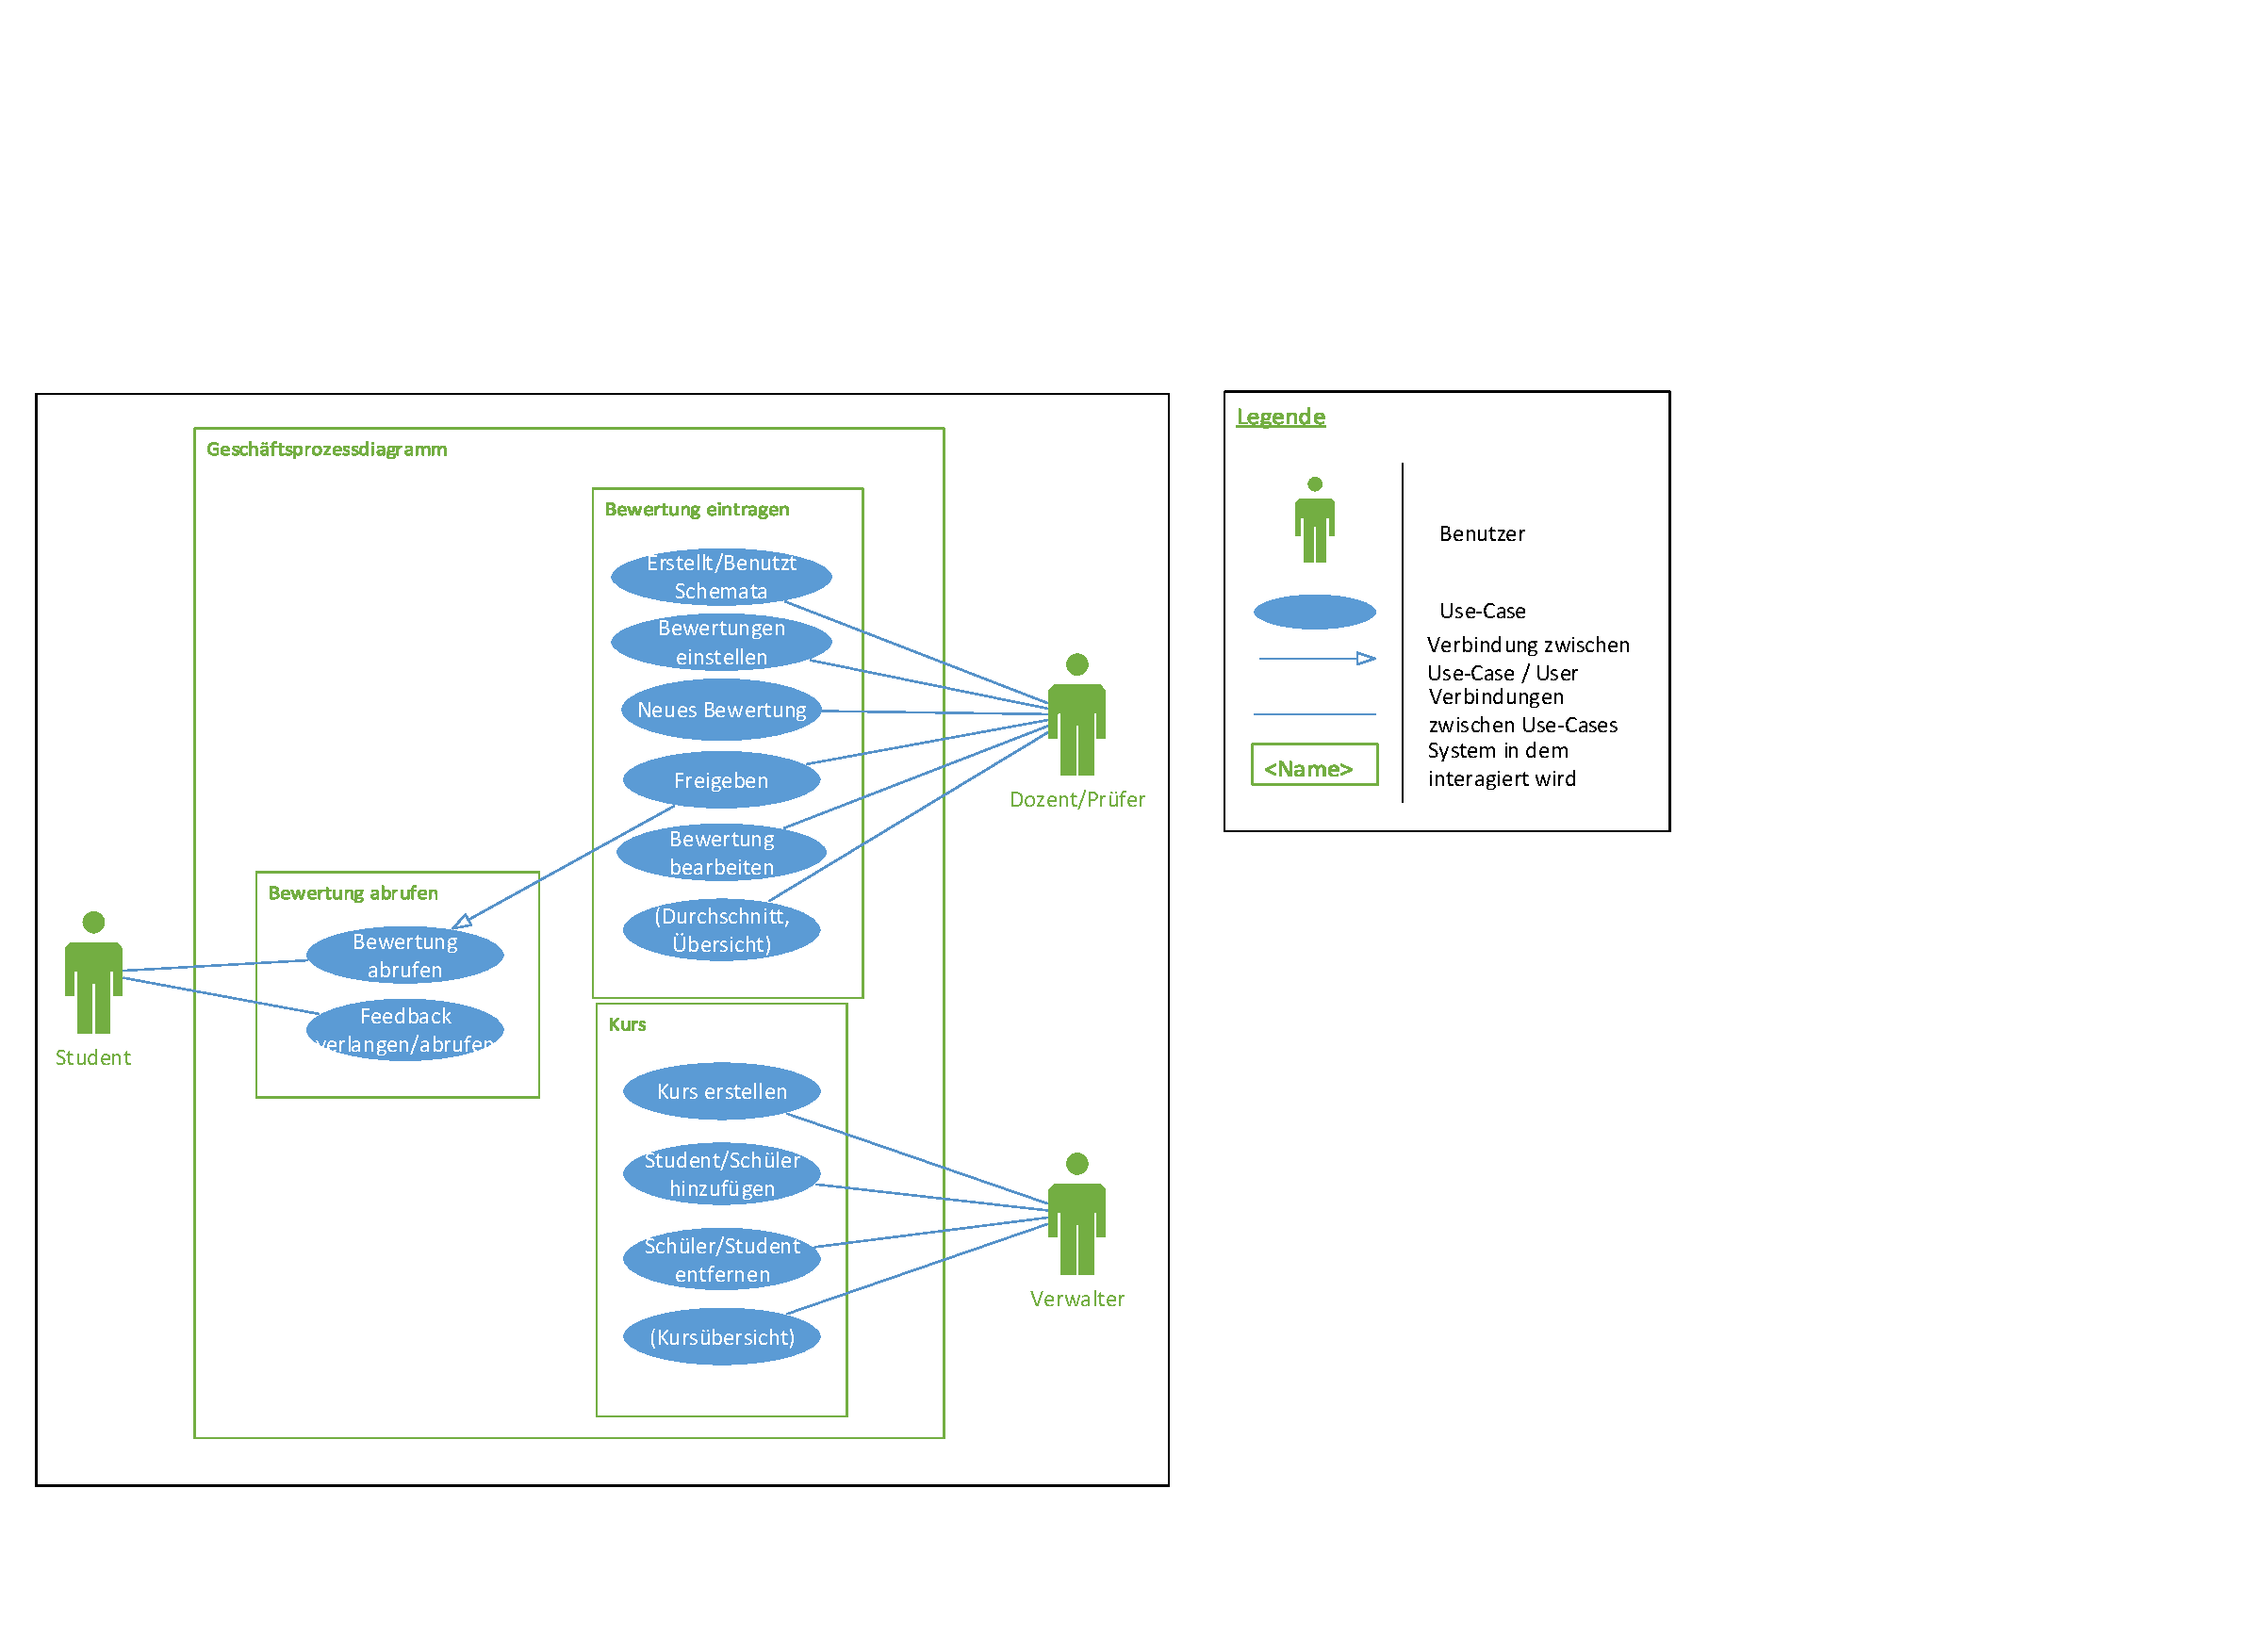
\includegraphics[width=0.99\textwidth]{../Diagramme/Use_Case.pdf}
		\caption{Use-Case Szenario}
		\label{fig:usecase}
	\end{figure}
	

% Produktfunktionen einfügen		
	\chapter{Produktfunktionen}

	% /LF10 Tabelle mit Programmstart/Login
	\begin{table}[H]
		\centering
		\caption{/LF10/Programmstart\_Login}
		\begin{tabularx}{\textwidth}{l|X}
			\toprule
			                        & Programmstart/Login                                         \\ \midrule
			Einstufung              & hoch                                                        \\
			Vorbedingungen          & Installation                                                \\
			Funktion erfolgreich    & Zugang zur Datenbank wird ermöglicht                        \\
			Funktion fehlgeschlagen & -                                                           \\
			Akteure                 & Student, Prüfer/Dozent, Verwaltung                          \\
			Auslöser                & System soll benutzt werden (Noten, Bewertungen, Verwaltung) \\
			Beschreibung            & 1. Benutzer startet das Programm                            \\
			                        & 2. Benutzer gibt Zugangsdaten ein                           \\
			                        & 3. System gibt Rückmeldung ob Login erfolgreich             \\
			Erweiterungen           & -                                                           \\
			Alternativen            & -                                                           \\ \bottomrule
		\end{tabularx}%
		\label{tab:LF10ProLogin}%
	\end{table}%
	
	% /LF20 Feedback erstellen
	\begin{table}[H]
		\centering
		\caption{/LF20/Feedback erstellen}
		\begin{tabularx}{\textwidth}{l|X}
			\toprule
			                        & Feedback erstellen                                                        \\ \midrule
			Einstufung              & mittel                                                                    \\
			Vorbedingungen          & Bewertungen müssen erstellt sein                                          \\
			Funktion erfolgreich    & Feedback kann eingetragen werden                                          \\
			Funktion fehlgeschlagen & Feedback kann nicht eingetragen werden                                    \\
			Akteure                 & Dozenter/Prüfer                                                           \\
			Auslöser                & Feedback ist erwünscht bzw. wird gegeben                                  \\
			Beschreibung            & 1. Prüfer wählt Bewertung aus zu welcher ein Feedback gegeben werden soll \\
			                        & 2. Prüfer trägt Feedback in Textfeld ein                                  \\
			                        & 3. Prüfer schickt Feedback an System ab                                   \\
			Erweiterungen           & -                                                                         \\
			Alternativen            & Persönlich fragen                                                         \\ \bottomrule
		\end{tabularx}%
		\label{tab:LF20createFB}%
	\end{table}%
	
	% /LF30 Feedback abrufen
	\begin{table}[H]
		\centering
		\caption{/LF30/Feedback abrufen}
		\begin{tabularx}{\textwidth}{l|X}
			\toprule
			                        &                           Feedback abrufen \\ \midrule
			             Einstufung &                                     mittel \\
			         Vorbedingungen &                Feedback muss erstellt sein \\
			   Funktion erfolgreich &             Feedback kann abgerufen werden \\
			Funktion fehlgeschlagen &     Feedback kann nicht eingetragen werden \\
			                Akteure &                                    Student \\
			               Auslöser &   Feedback ist erwünscht bzw. wird gegeben \\
			           Beschreibung &        1. Student hat Feedback angefordert \\
			                        &                  2. Feedback wurde gegeben \\
			                        & 3. Student kann gegebenes Feedback abrufen \\
			          Erweiterungen &                                          - \\
			           Alternativen &                          Persönlich fragen \\ \bottomrule
		\end{tabularx}%
		\label{tab:LF30holeFB}%
	\end{table}%
	
	% /LF40 Bewertungsschema erstellen
	\begin{table}[H]
		\centering
		\caption{/LF40/Bewertungsschema erstellen}
		\begin{tabularx}{\textwidth}{l|X}
			\toprule
			                        &               Bewertungsschema erstellen \\ \midrule
			             Einstufung &                                     hoch \\
			         Vorbedingungen &                          Schema erfinden \\
			   Funktion erfolgreich &                  Schema wird gespeichert \\
			Funktion fehlgeschlagen &                                        - \\
			                Akteure &                          Dozente/Prüfer \\
			               Auslöser &     Prüfer will neue Bewertung erstellen \\
			           Beschreibung & 1. Prüfer muss Bewertungskriterien haben \\
			                        &  2. Prüfer trägt Bewertungskriterien ein \\
			                        &            3. Prüfer speichert Schema ab \\
			          Erweiterungen &                                        - \\
			           Alternativen &                        Persönlich fragen \\ \bottomrule
		\end{tabularx}%
		\label{tab:LF40createBewSchem}%
	\end{table}%
	
	% Table generated by Excel2LaTeX from sheet 'Tabelle5'
	\begin{table}[H]
		\centering
		\caption{/LF50/Bewertung abrufen}
		\begin{tabularx}{\textwidth}{l|X}
			\toprule
			                        &                                          Bewertung abrufen \\ \midrule
			             Einstufung &                                                       hoch \\
			         Vorbedingungen &                           Bewertungen müssen erstellt sein \\
			   Funktion erfolgreich &                                   Bewertung wird abgerufen \\
			Funktion fehlgeschlagen &                                                          - \\
			                Akteure &                                        Student, Verwaltung \\
			               Auslöser &                      Bewertung für Student wurde abgegeben \\
			           Beschreibung & 1.Student bekommt Information dass Bewertung verfügbar ist \\
			                        &                               2. Student ruft Bewertung ab \\
			          Erweiterungen &                                                          - \\
			           Alternativen &                                          Persönlich fragen \\ \bottomrule
		\end{tabularx}%
		\label{tab:LF50holeBew}%
	\end{table}%
	
	% Bewertung eintragen (H2)
	\begin{table}[H]
		\centering
		\caption{/LF60/Bewertung eintragen (H2)}
		\begin{tabularx}{\textwidth}{l|X}
			\toprule
			                        &                     Bewertung eintragen (H2) \\ \midrule
			             Einstufung &                                         hoch \\
			         Vorbedingungen &                    Schema muss erstellt sein \\
			   Funktion erfolgreich &            Bewertung wird Schema hinzugefügt \\
			Funktion fehlgeschlagen &            Automatisch schlechtere Bewertung \\
			                Akteure &                              Dozenter/Prüfer \\
			               Auslöser &  Prüfer Bewertet einzelne Punkte des Schemas \\
			           Beschreibung &        1. Prüfer wählt erstelltes Schema aus \\
			                        &         2. Prüfer bewertet nach H2 Kriterium \\
			                        & 3. Schema mit Bewertungen wird abgespeichert \\
			          Erweiterungen &                                            - \\
			           Alternativen &                                            - \\ \bottomrule
		\end{tabularx}%
		\label{tab:LF60eintrBew}%
	\end{table}%
	
	\begin{table}[H]
		\centering
		\caption{/LF70/Score S2R}
		\begin{tabularx}{\textwidth}{l|X}
			\toprule
			                        & Score S2R                                        \\ \midrule
			Einstufung              & hoch                                             \\
			Vorbedingungen          & H2 ist vorhanden                                 \\
			Funktion erfolgreich    & Berechnung ist erfolgreich                       \\
			Funktion fehlgeschlagen & -                                                \\
			Akteure                 & Dozenter/Prüfer                                  \\
			Auslöser                & Prüfer will Bewertung ausrechnen                 \\
			Beschreibung            & 1. Prüfer muss H2 Bewertung einstellen           \\
			                        & 2. Das Programm berechnet eine Rate              \\
			                        & 3. Rate wird abgespeichert                       \\
			Erweiterungen           & Weitere Parameters / Impacts (R2S) können folgen \\
			Alternativen            & -                                                \\ \bottomrule
		\end{tabularx}%
		\label{tab:LF70S2R}%
	\end{table}%

	% Score R2S
	\begin{table}[H]
		\centering
		\caption{/LF80/Score R2S }
		\begin{tabularx}{\textwidth}{l|X}
			\toprule
			                        & Score R2S                                                            \\ \midrule
			Einstufung              & hoch                                                                 \\
			Vorbedingungen          & S2R ist vorhanden                                                    \\
			Funktion erfolgreich    & Weitere Parameters / Impacts sollen in den Score eingerechnet werden \\
			Funktion fehlgeschlagen & -                                                                    \\
			Akteure                 & Dozenter/Prüfer                                                      \\
			Auslöser                & Prüfer will weitere Parameters einbinden                             \\
			Beschreibung            & 1. Prüfer muss S2R besitzen                                          \\
			                        & 2. Das Programm berechnet weite Parameters / Impacts                 \\
			                        & 3. Neue Rate wird abgespeichert                                      \\
			Erweiterungen           & -                                                                    \\
			Alternativen            & -                                                                    \\ \bottomrule
		\end{tabularx}%
		\label{tab:LF80R2S}%
	\end{table}%
	
% Produktdaten
	\chapter{Produktdaten}
	In den Produktdaten sollten enthalten sein:
	\begin{itemize}
		\item Name des Studenten
		\item Vorname des Studenten
		\item Matrikelnummer des Studenten
		\item Die "`Endscores"' des Studenten
		\item "`Zwischenscores"' 
		\item Fach vom Score 
		\item Name des Dozenten / Prüfer
		\item Vorname des Dozenten / Prüfer
		\item Dozenten\_ID / Prüfer\_ID
		\item Score - Schemata
		\item Prüfmuster

	\end{itemize}
	Insgesamt können von jedem Studenten mehrere Score eingetragen werden. Name, Vorname und Matrikelnummer sind nur einmal in der Datenbank hinterlegt um Redundanz zu verhindern. 
	Die Datenbank sollte so dimensioniert werden, damit alle Datei genug Speicher besitzen bzw. folgende Daten ohne Problem gespeichert werden können. Als Richtwert werden ca. 10.000 Einträge gewählt. 
	
% Produktleistungen
	\chapter{Produktleistungen}
	Die Software soll eine Stabilität enthalten, wodurch mehrere Studenten/Dozenten auf einmal darauf zugreifen können. Die Qualitätsanforderung sind Vormaussetzung um ein voll funktionsfähig Programm zu erstellen. Es müssen Schwerpunkte in diesem Programm gelegt werden.\\
	
	Es muss zwischen Funktionalität und Nicht-funktionale Anforderung unterschieden werden. Die Funktionalität ist entscheiden für das Programm. Nicht-funktionale Anforderung sind im ersten Schritt für das Grundprogramm nicht wichtig, können jedoch bei genügend Zeit hinzugefügt werden.\\
	
	Es wurde die ISO / IES Norm 9126 gewählt, um die Softwarequalität sicherzustellen. Diese Norm bezieht sich sehr auf die Qualität der Software als Produkt. Die Produktqualität ist entscheidend, damit das Programm voll funktionsfähig sein wird. 


% Qualitätsanforderungen
	\chapter{Qualitätsanforderungen}

%Qualitätsanforderungen	
\begin{table}[H]
	\centering
	\caption{Qualitätsanforderungen}
	\begin{tabularx}{\textwidth}{l|X|X|X|X}
		\toprule
		\textbf{Produktqualität}       & \centering \textbf{sehr gu}t & \centering \textbf{gut}      & \centering \textbf{normal}   & \textbf{irrelevant} \\
		\toprule
		\multicolumn{5}{l}{\textbf{Funktionalität}}                           \\ 
		\midrule
		\quad Angemessenheit        &          &          & $\times$ &  \\ \hline
		\quad Richtigkeit           &          &  $\times$ &          &  \\ \hline
		\quad Interoperabilität     &          &          & $\times$ &  \\ \hline
		\quad Ordnungsmäßigkeit     &          & $\times$ &          &  \\ \hline
		\quad Sicherheit            &          & $\times$ &          &  \\
		\toprule
		\multicolumn{5}{l}{\textbf{Zuverlässigkeit}}                          \\
		\midrule
		\quad Reife                 &          & $\times$ &          &  \\ \hline
		\quad Fehlertolleranz       &          &          & $\times$ &  \\ \hline
		\quad Wiederherstellbarkeit &          &          & $\times$ &  \\ 
		\toprule
		\multicolumn{5}{l}{\textbf{Benutzbarkeit}}                            \\ 
		\midrule
		\quad Verständlichkeit      & $\times$ &          &          &  \\ \hline
		\quad Erlernbarkeit         & $\times$ &          &          &  \\ \hline
		\quad Bedienbarkeit         & $\times$ &          &          &  \\ 
		\toprule
		\multicolumn{5}{l}{\textbf{Effizienz}}                                \\
		\midrule
		\quad Zeitverhalten         &          &          &          & $\times$       \\ \hline
		\quad Verbrauchsverhalten   &          &          & $\times$ &  \\ 
		\toprule
		\multicolumn{5}{l}{\textbf{Änderbarkeit}}                             \\ 
		\midrule
		\quad Analysierbarkeit      &          &          & $\times$ &  \\ \hline
		\quad Modifizierbarkeit     &          &          &          & $\times$       \\ \hline
		\quad Stabilität            &          &          & \centering  $\times$ &  \\ \hline
		\quad Prüfbarkeit           &          &          & \centering $\times$ &  \\ 
		\toprule
		\multicolumn{5}{l}{\textbf{Übertragbarkeit}}                          \\ 
		\midrule
		\quad Anpassbarkeit         &          &          &          & $\times$       \\ \hline
		\quad Installierbarkeit     &          &          &          & $\times$       \\ \hline
		\quad Konformität           &          &          & $\times$ &  \\ \hline
		\quad Austauschbarkeit      &          &          &          & $\times$       \\ \hline
	\end{tabularx}%
	\label{tab:QualAnfor}%
\end{table}%
	
	\begin{itemize}
		\item Funktionalität:\\
		In der Rubrik Funktionalität spielt vor allem die Sicherheit eine große Rolle, weshalb die Qualitätsanforderungen hier sehr gut sein müssen. Es muss garantiert werden, dass keine Daten geklaut oder missbraucht werden können. Deshalb ist es ratsam hier mehr Zeit zu investieren. Die Punkte Richtigkeit und Ordnungsmäßigkeit müssen qualitativ nicht so hochwertig sein wie die Sicherheit, weil kleine Pannen bei der Benutzung keine gravierenden Schäden anrichten. Normale Qualität genügt bei Angemessenheit und Interoperabilität.\\
		
		\item Zuverlässigkeit:\\
		Insgesamt sollte das Programm zuverlässig laufen, jedoch müssen nicht überwiegend Ressourcen dafür verbraucht werden. Sollte das System abstürzen oder nicht ordnungsgemäß laufen, kann man nach einem Neustart weiterarbeiten.\\
		
		\item Benutzbarkeit:\\
		Viel Augenmerk wird auf die Benutzbarkeit gelegt. Das Programm sollte für den Anwender einfach zu bedienen sein und sich selbst erklären, damit keine Schulung mehr notwendig ist. \\
		
		\item 	Effizienz:\\
		Ausschlaggebend ist die Effizienz nicht, da das Bewertungssystem nicht besonders schnell die Score abrufen und verarbeiten muss. \\
		
		\item Änderbarkeit:		
		Für die Zukunft können weitere Features eingebaut werden, wenn man möchte. Grundsteine für weitere Features werden nicht gezielt gelegt.\\
					
		\item  Übertragbarkeit:
		Die Übertragbarkeit spielt eine untergeordnete Rolle, da man nur drauf zugreifen muss. Installieren oder ähnliches muss nicht getan werden. \\
			
	\end{itemize}	
	
% Benutzungsoberfläche
	\chapter{Benutzungsoberfläche}
	Die Thema wird anfangs absichtlich etwas vernachlässigt. Das Design ist für funktionsfähig des Programmes erstmal nicht entscheidend.
	\begin{itemize}
 
		\item Desktop-Programm-Design nach "Java Look and Feel Design Guidelines"
		\item IOs App nach "Apple Design Guidelines"
	\end{itemize}
	
	
% Technische Produktumgebung
	\chapter{Technische Produktumgebung}
	Auf dem Server wird eine CouchDB-Datenbank verwendet. Auf der Clientseite wird ein Java–Programm installiert.
	
	\section{Software}
	\begin{itemize}
		\item Betriebssystem : Windows 7, Windows 8, Windows 8.1, Mac OS X
		\item Laufzeitsystem: Als Laufzeitsystem wird ein \ac{JRE} benötigt, welches für die meisten Betriebssysteme von Oracle zur Verfügung gestellt wird. \footnote{http://www.oracle.com/technetwork/java/index.html}
		\item Datenbank: Apache CouchDB\footnote{http://couchdb.apache.org}\\
			Apache CouchDB ist ein NoSQL Datenbanksystem von Apache, welche mittels \ac{JSON} die einzelnen Dokumente hinterlegt. Als API stellt CouchDB \ac{HTTP} zur Verfügung. Daher ist CouchDB speziell für Anwendungen entwickelt, welche mit dem Internet verbunden sind und über dieses kommunizieren. CouchDB kann einfach mittels den von Apache bereitgestellten Paketen auf jedem System installiert werden. Es wird Windows, Linux wie auch Mac OSX unterstützt. 
		\item Client: Java Programm
			Als Clientsoftware wird ein Java-Programm benötigt. Es wird Java verwendet, da es auf den meisten Geräten läuft.
	\end{itemize}

	\section{Hardware}
	\begin{itemize}
		\item \underline{Server:} \\
			Die Hardware des Servers muss performant genug sein, um die  	CouchDB lauffähig auf dem System zu halten. Es wird mindestens ein 32-Bit Betriebssystem benötigt.
		
		\item \underline{Client:}\\
			Die Mindestanforderungen für die Clients sind ein lauffähiges \ac{JRE}, welches auf den meisten Betriebssystemen von Oracle zur Verfügung gestellt wird.
	\end{itemize}

	\section{Orgware}
	Der Server muss mit dem Internet verbunden sein. Es wird empfohlen dies über eine synchrone Standleitung (10TBit/s) zu realisieren, um immer verfügbar zu sein.\\
	Die Clients müssen ebenfalls mit dem Internet verbunden sein. Es wird mindestens 2Mbit/s empfohlen.
	
	\section{Produkt-Schnittstellen}
	Anbindung von Java und CoucDB über JSON.
	
	
% Anforderungen an die Entwicklungsumgebung
	\chapter{Spezielle Anforderungen an die Entwicklungs-Umgebung}
	
	\section{Software}
	Als Software für die Entwicklung wird Windows 7 und Mac OSX 10.10 verwendet, da diese Systeme zur Verfügung stehen. Des weiteren wird Eclipse als IDE für Java verwendet. Um die Daten abzulegen wird eine CouchDB Datenbank verwendet.
	Da wir in der Vergangenheit sehr gute Ergebnisse mit Java erzielt haben und eine CouchDB-Datenbank für dieses Projekt sehr sinnvoll erscheint, da es mit der Datenmenge gut zurecht kommt und noch performant genug ist.
	\section{Hardware}
	Windows 7\\
	
	\textbf{	MacBook Pro (13 Zoll, Mitte 2009)}\\
	\textbf{Prozessor} 	\quad 2,26GHz Intel Core 2 Duo\\
	\textbf{Speicher} 	\quad 4GB 1067 MHz DDR3\\
	\textbf{Betriebsystem}\quad OSX 10.Yosemite

	
	\section{Orgware}
	Internet Zugang
	
	\section{Produkt-Schnittstellen}
	Internetanbindung von Java und CouchDB Datenbank.
		
% Gliederung in Teilprodukte
	\chapter{Gliederung in Teilprodukte}
	Drei Teilprodukte die nacheinander fertiggestellt werden. Die zweistufige holistische Bewertung (H2) / Rate-to-Score (R2S) sowie Score-to-Rate (S2R) soll als erstes fertiggestellt werden, damit soll die Kernfunktionalität vorhanden ist. \\
	Der zweite Schritt ist die Datenbankanbindung inkl. der Benutzerauthentifizierung.\\
	Der letzte Schritt ist die Benutzerschnittstelle (GUI). Für die Desktop Version muss eine andere Gui erstellt werden als für die Mobile Version.


%\chapter{Ergänzungen}	
%	In diesem Kapitel werden Ergänzungen sowie spezielle Anforderungen beschrieben die über die aufgeführten Kapitel 1 bis 12 hinausgehen. Beispielsweise können hier Installationsbedingungen festgelegt werden wie:\\
%	bauliche und räumliche Voraussetzungen\\
%	Bereitstellung von Testdaten\\
%	Bereitstellung von Hilfspersonal\\
%	Außerdem können hier zu berücksichtigende\\
%	Normen\\
%	Vorschriften\\
%	Patente und\\
%	Lizenzen aufgeführt werden.

% Anhang auf neuer Seite
\newpage
\appendix

\setcounter{page}{1}
\renewcommand{\thepage}{\arabic{page}}

% Anhang
	\chapter{Anhang}
\appendix
	\section{Begriffsdefinitionen}

	\section{Abkürzungsverzeichnis}
		\begin{acronym} 
			% Acronym mit \acro hinzu
			\acro{API}{Application Programming Interface (Programmierschnittstelle)}
			\acro{Add-On}{Erweiterungspaket}
			\acro{JRE}{Java Runtime Environement}
			\acro{JSON}{JavaScript Object Notation}
			\acro{HTTP}{Hypertext Transfer Protocol}
		\end{acronym}
	
	% Abbildungsverzeichnis
	\listoffigures
	
	\section{Aufwandsabschätzung}
	%Aufwandsabschätzungstabelle einfügen

	\begin{figure}
		\centering
		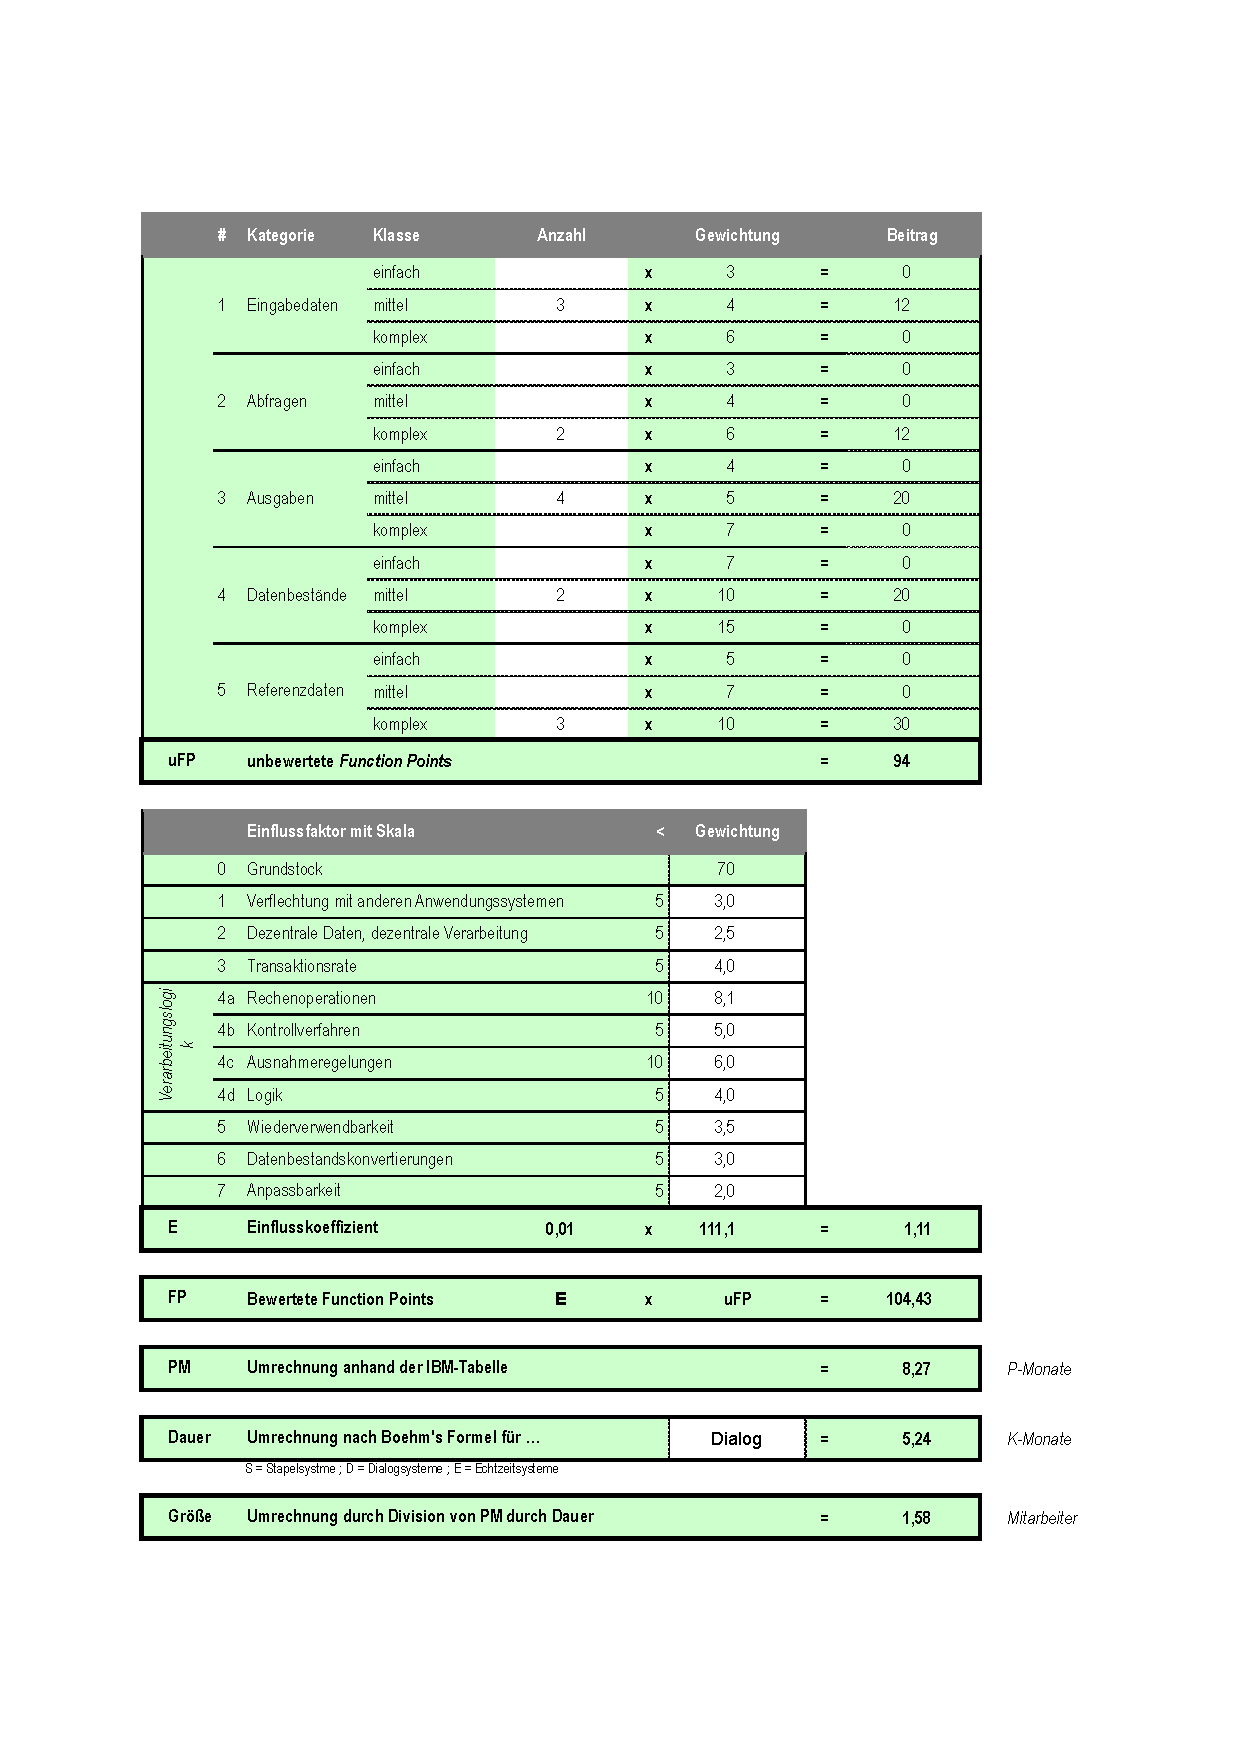
\includegraphics[width=0.9\textwidth]{data/Aufwandsabschaetzung.pdf}
		\caption{Aufwandsabschätzungen}
	\end{figure}
	
	\section{Datenflussdiagramme sowie weitere Diagramme}

	\begin{figure}[H]
		\centering
		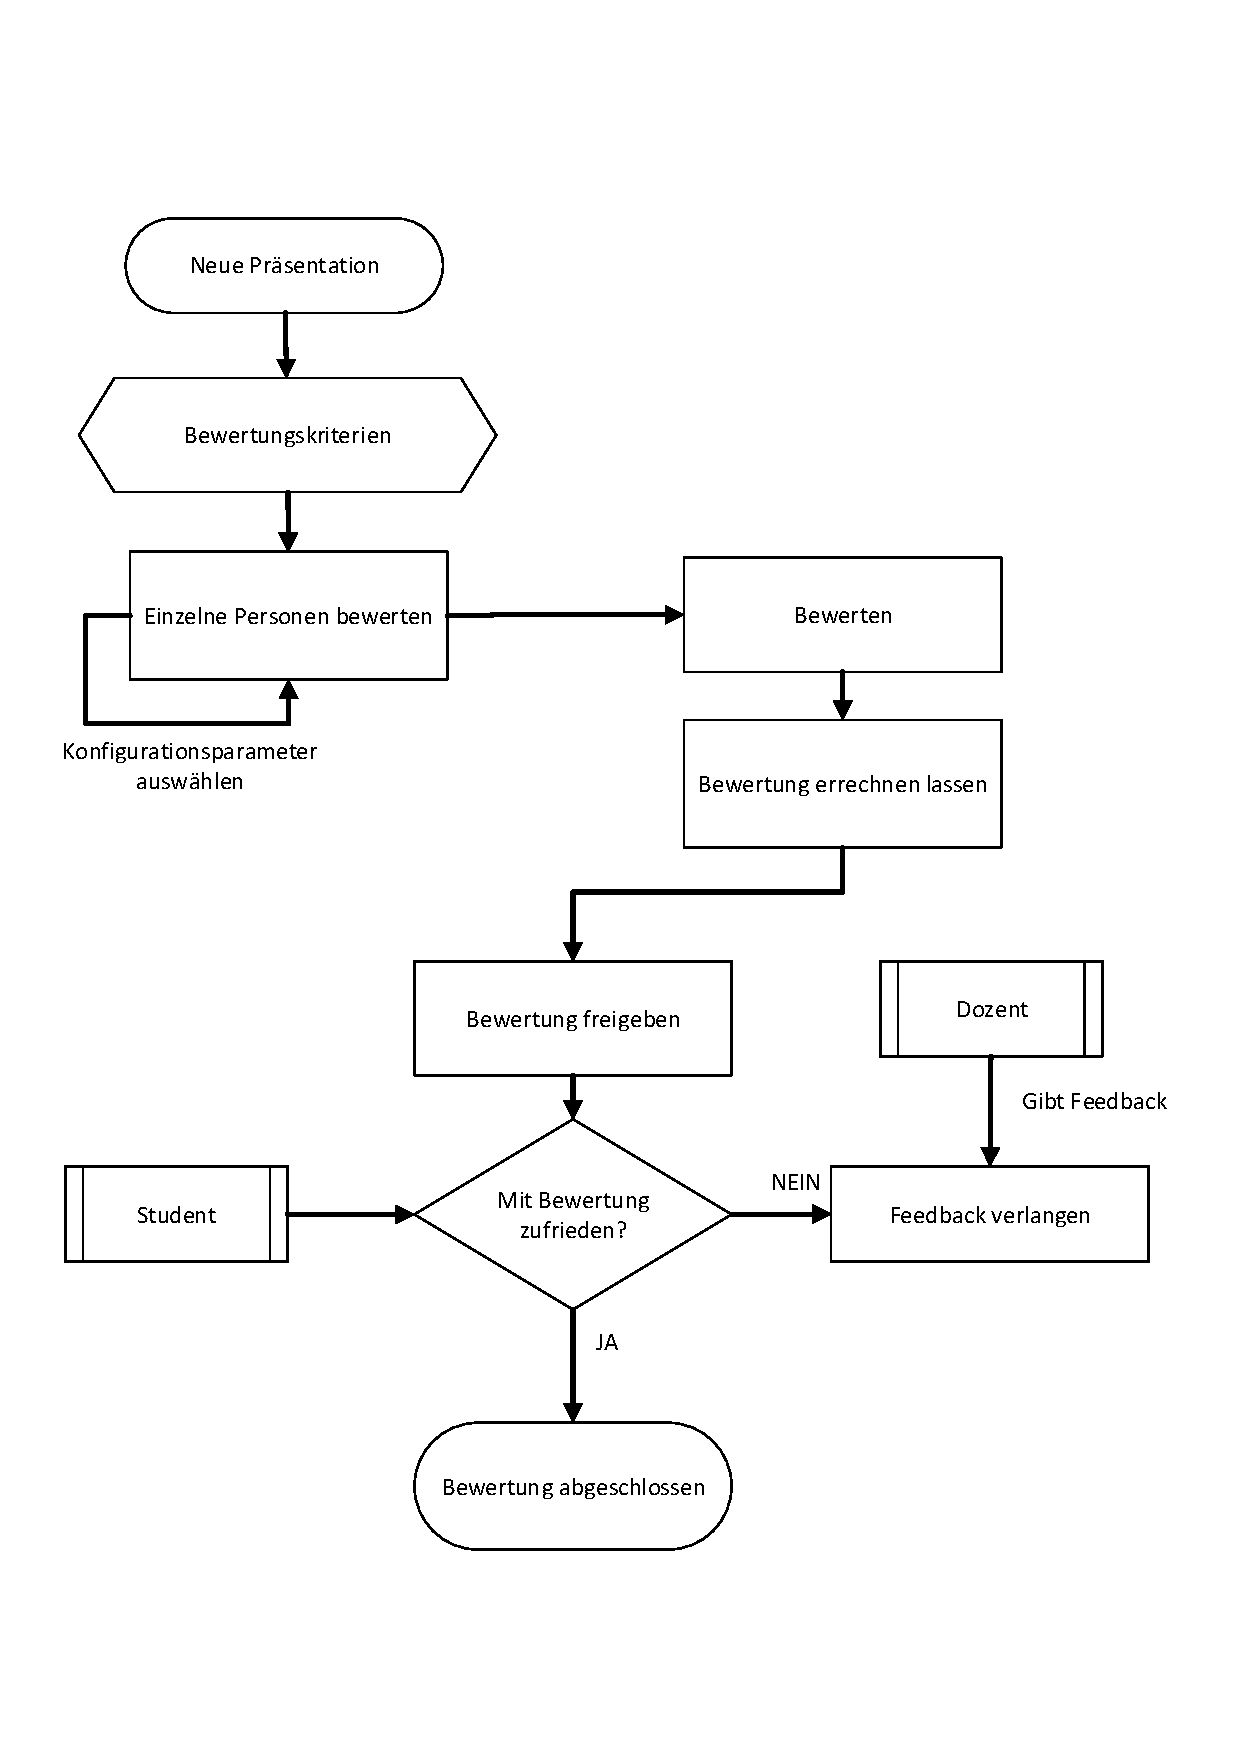
\includegraphics[height=0.9\textheight]{../Diagramme/Beispiel-FlussdiagrPraesi.pdf}
		\caption{Beispielprozess einer Bewertung einer Präsentation}
	\end{figure}
	\begin{figure}[H]
		\centering
		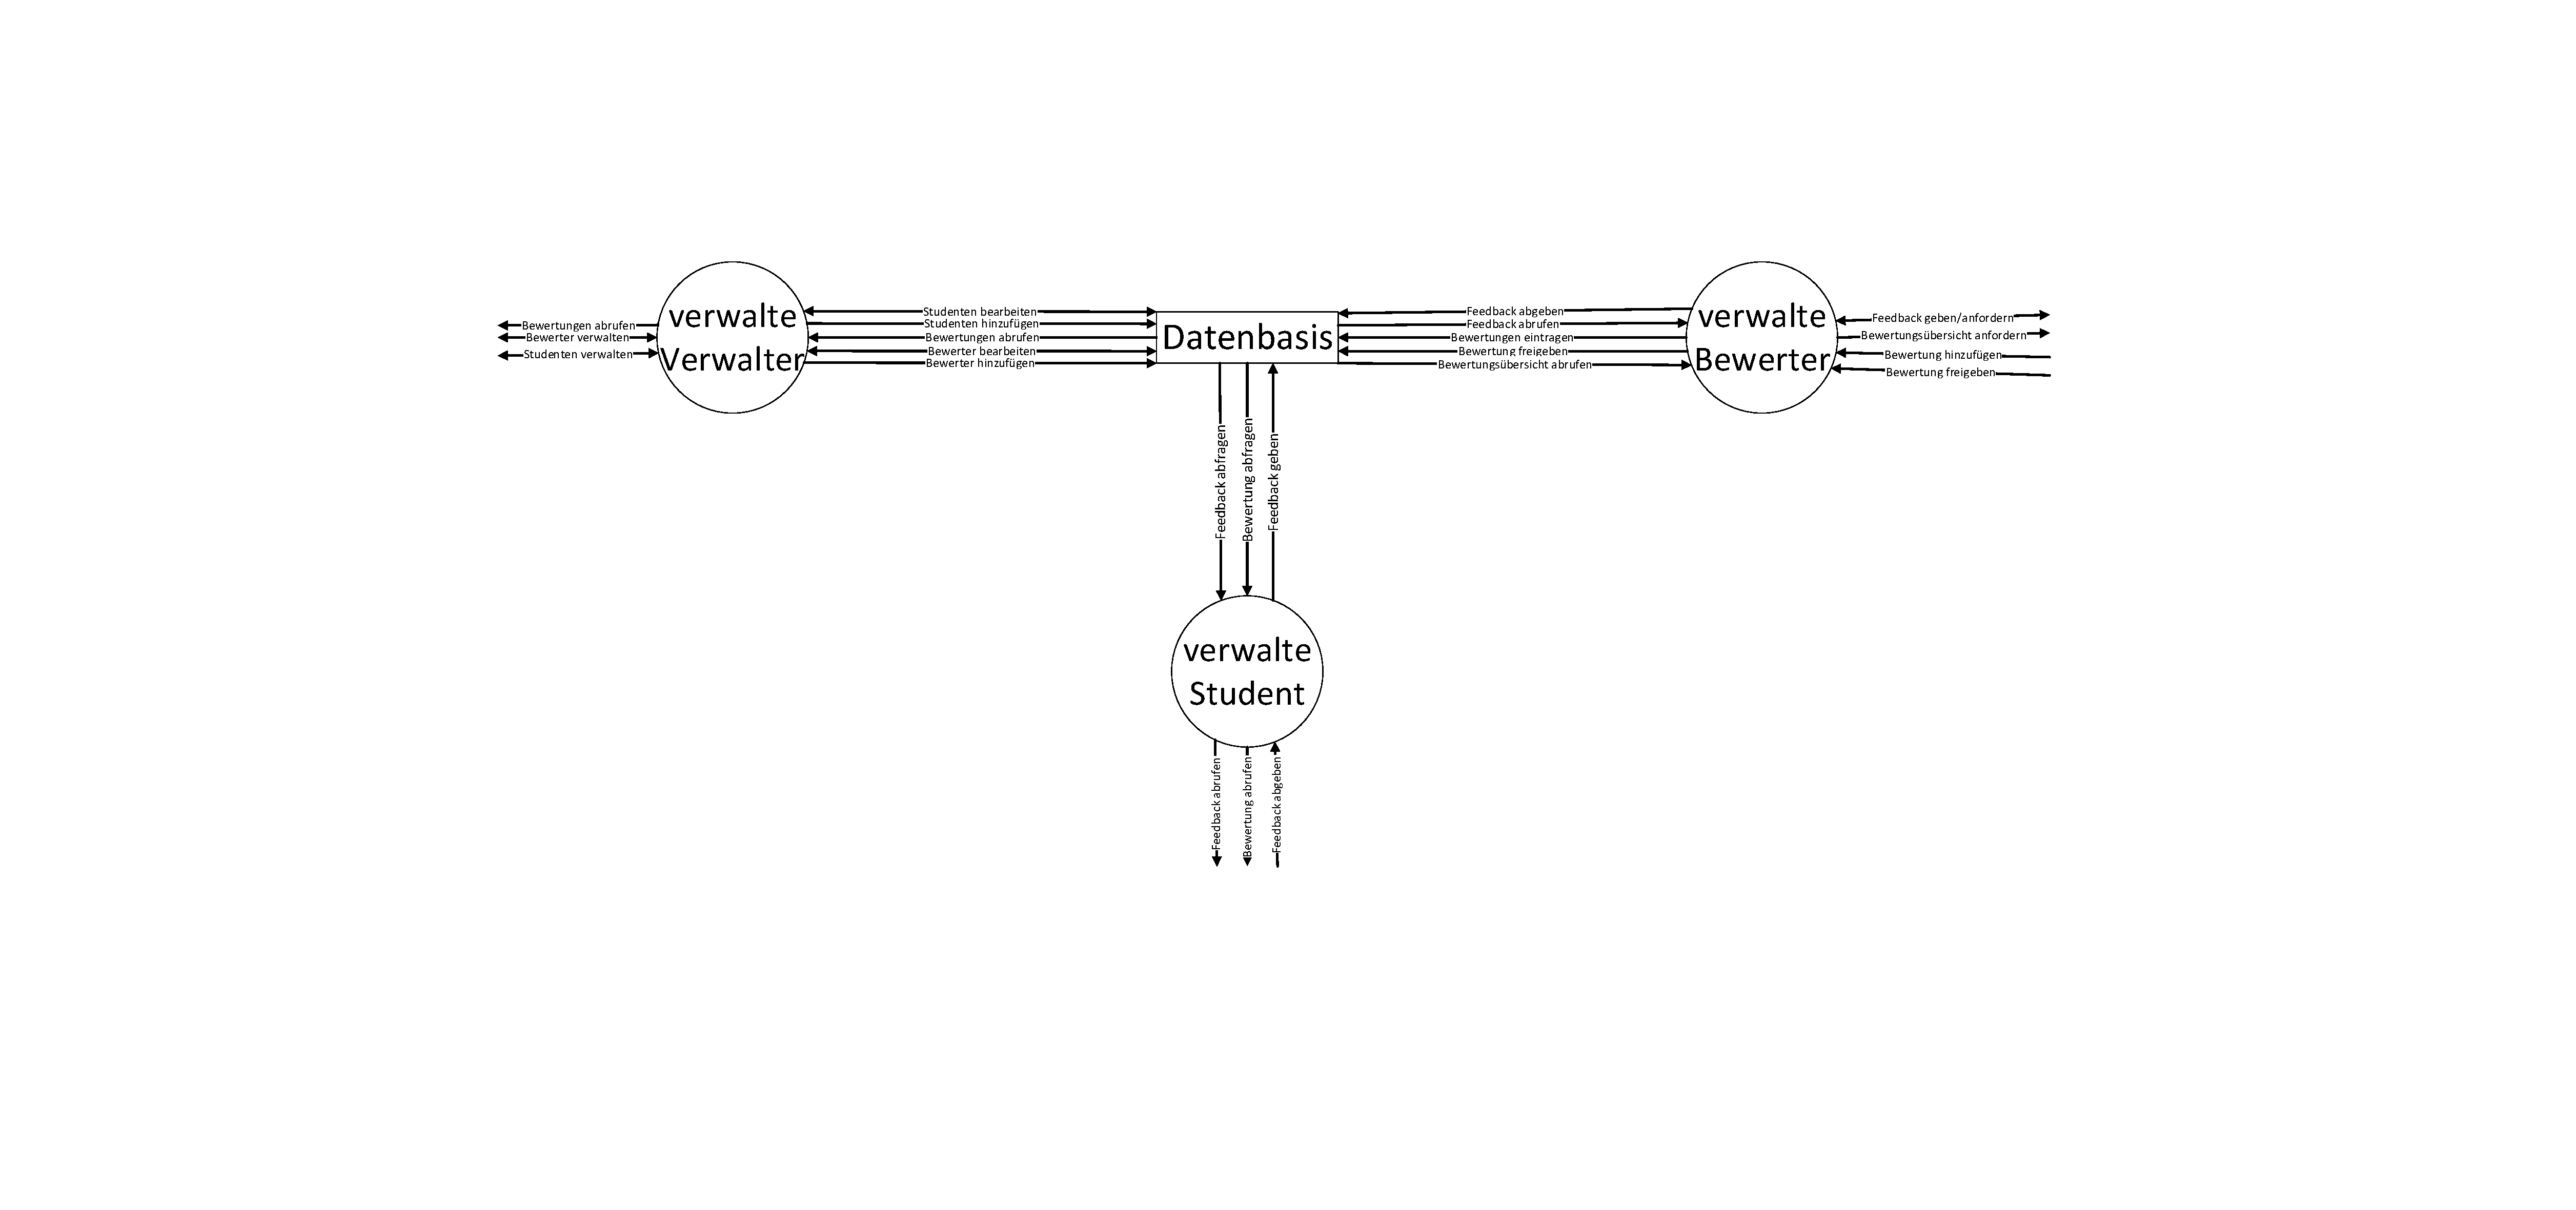
\includegraphics[width=1.4\textwidth, angle=90, origin=c]{../Diagramme/Kontextdiagramm_DFD0.pdf}
		\caption{Kontextdiagramm}
	\end{figure}
	\begin{figure}[H]
		\centering
		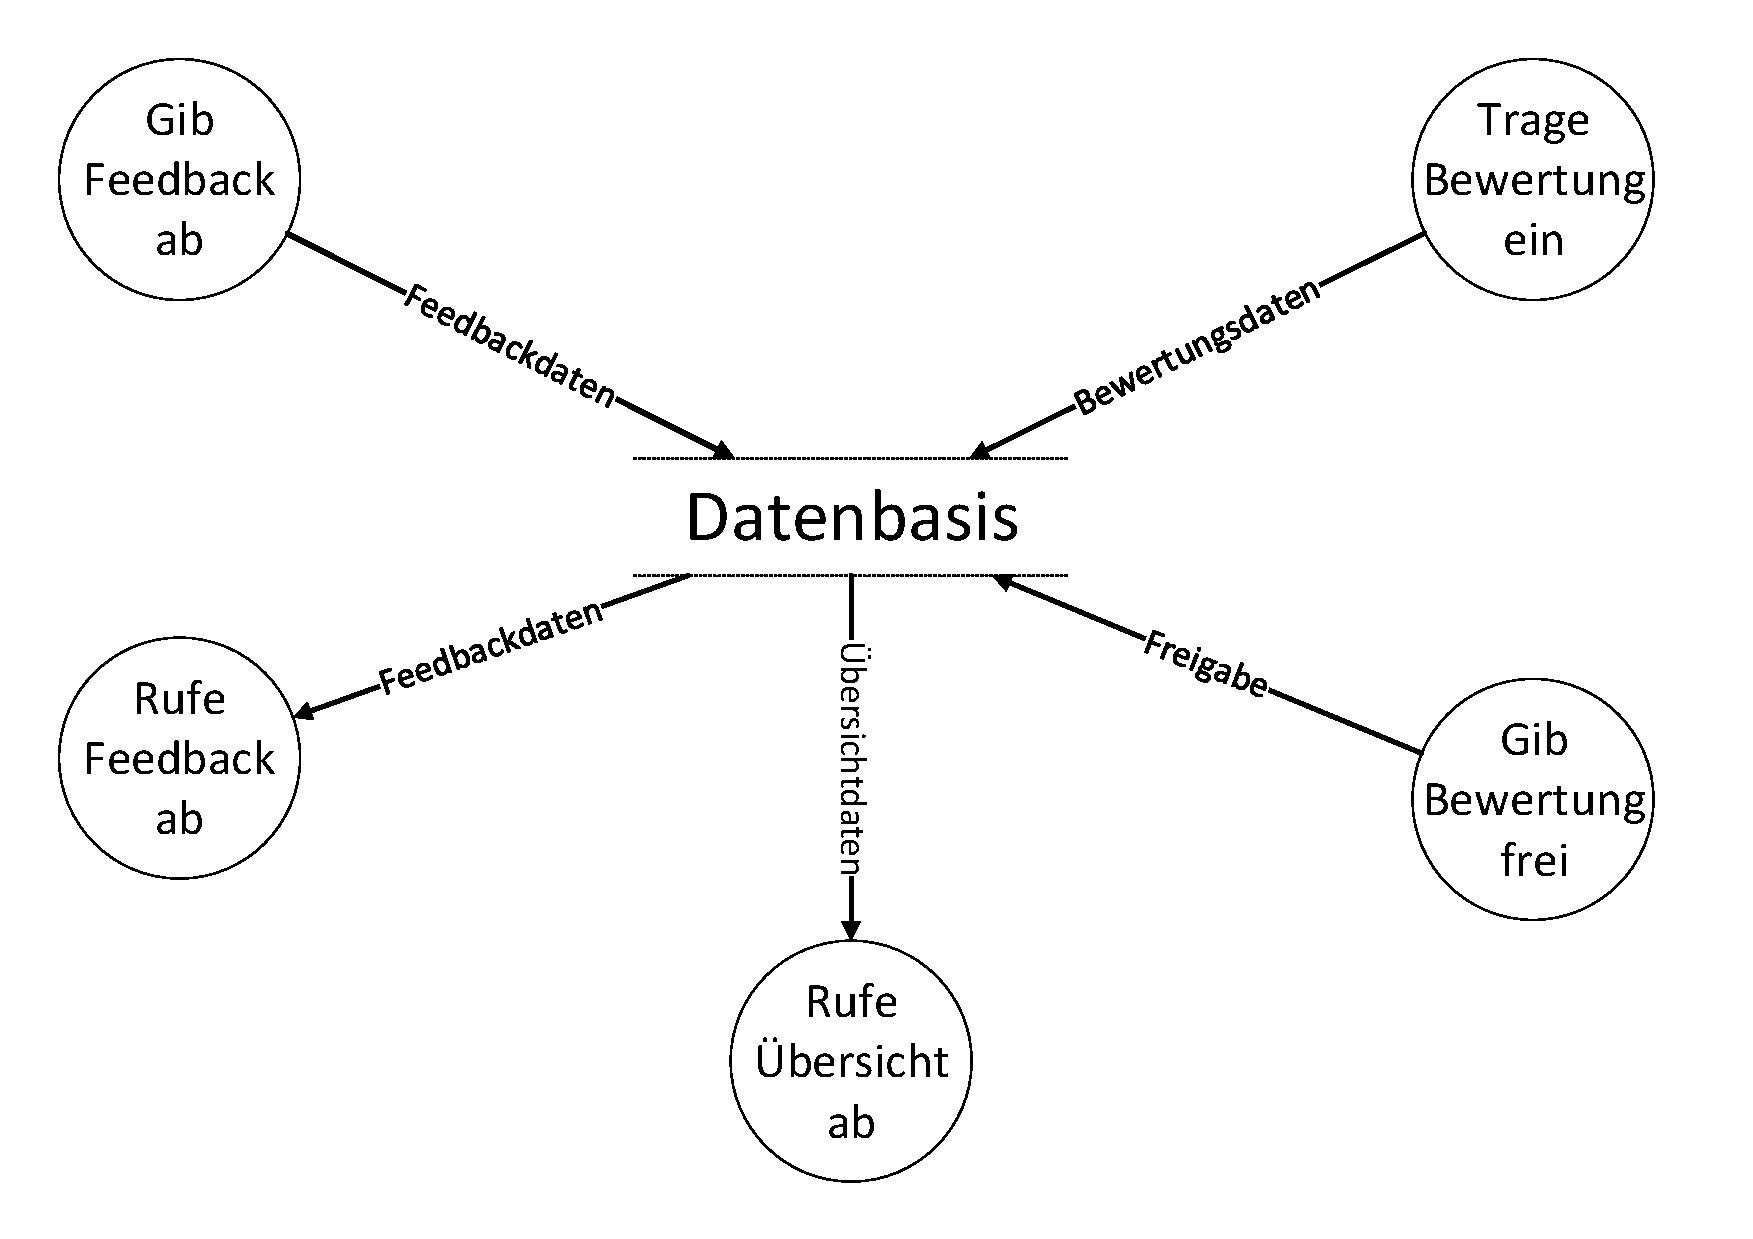
\includegraphics[width=1.4\textwidth, angle=90, origin=c]{../Diagramme/Kontextdiagramm_DFD2_Bewerter.pdf}
		\caption{Datenflussdiagramm Bewerter}
	\end{figure}
	\begin{figure}[H]
		\centering
		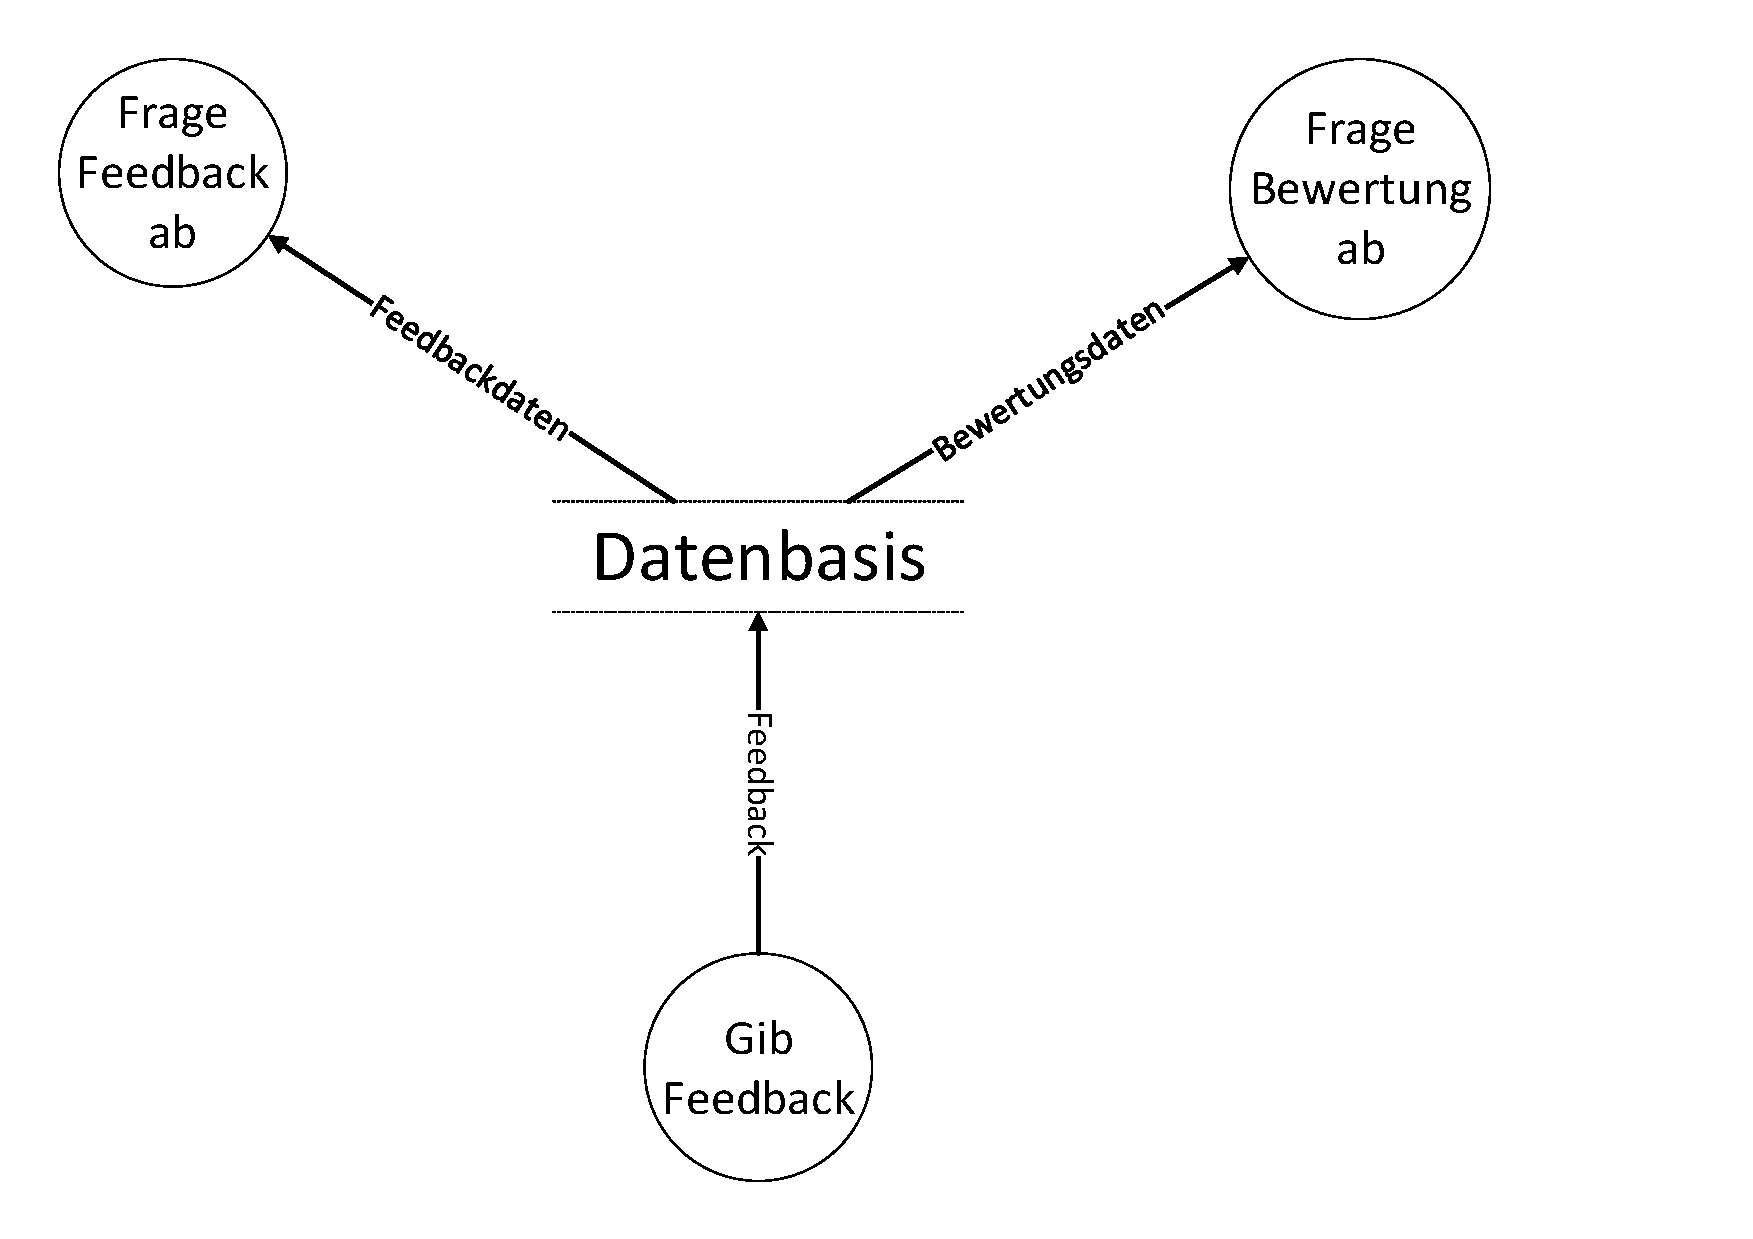
\includegraphics[width=1.4\textwidth, angle=90, origin=c]{../Diagramme/Kontextdiagramm_DFD2_Student.pdf}
		\caption{Datenflussdiagramm Student}
	\end{figure}
	\begin{figure}[H]
		\centering
		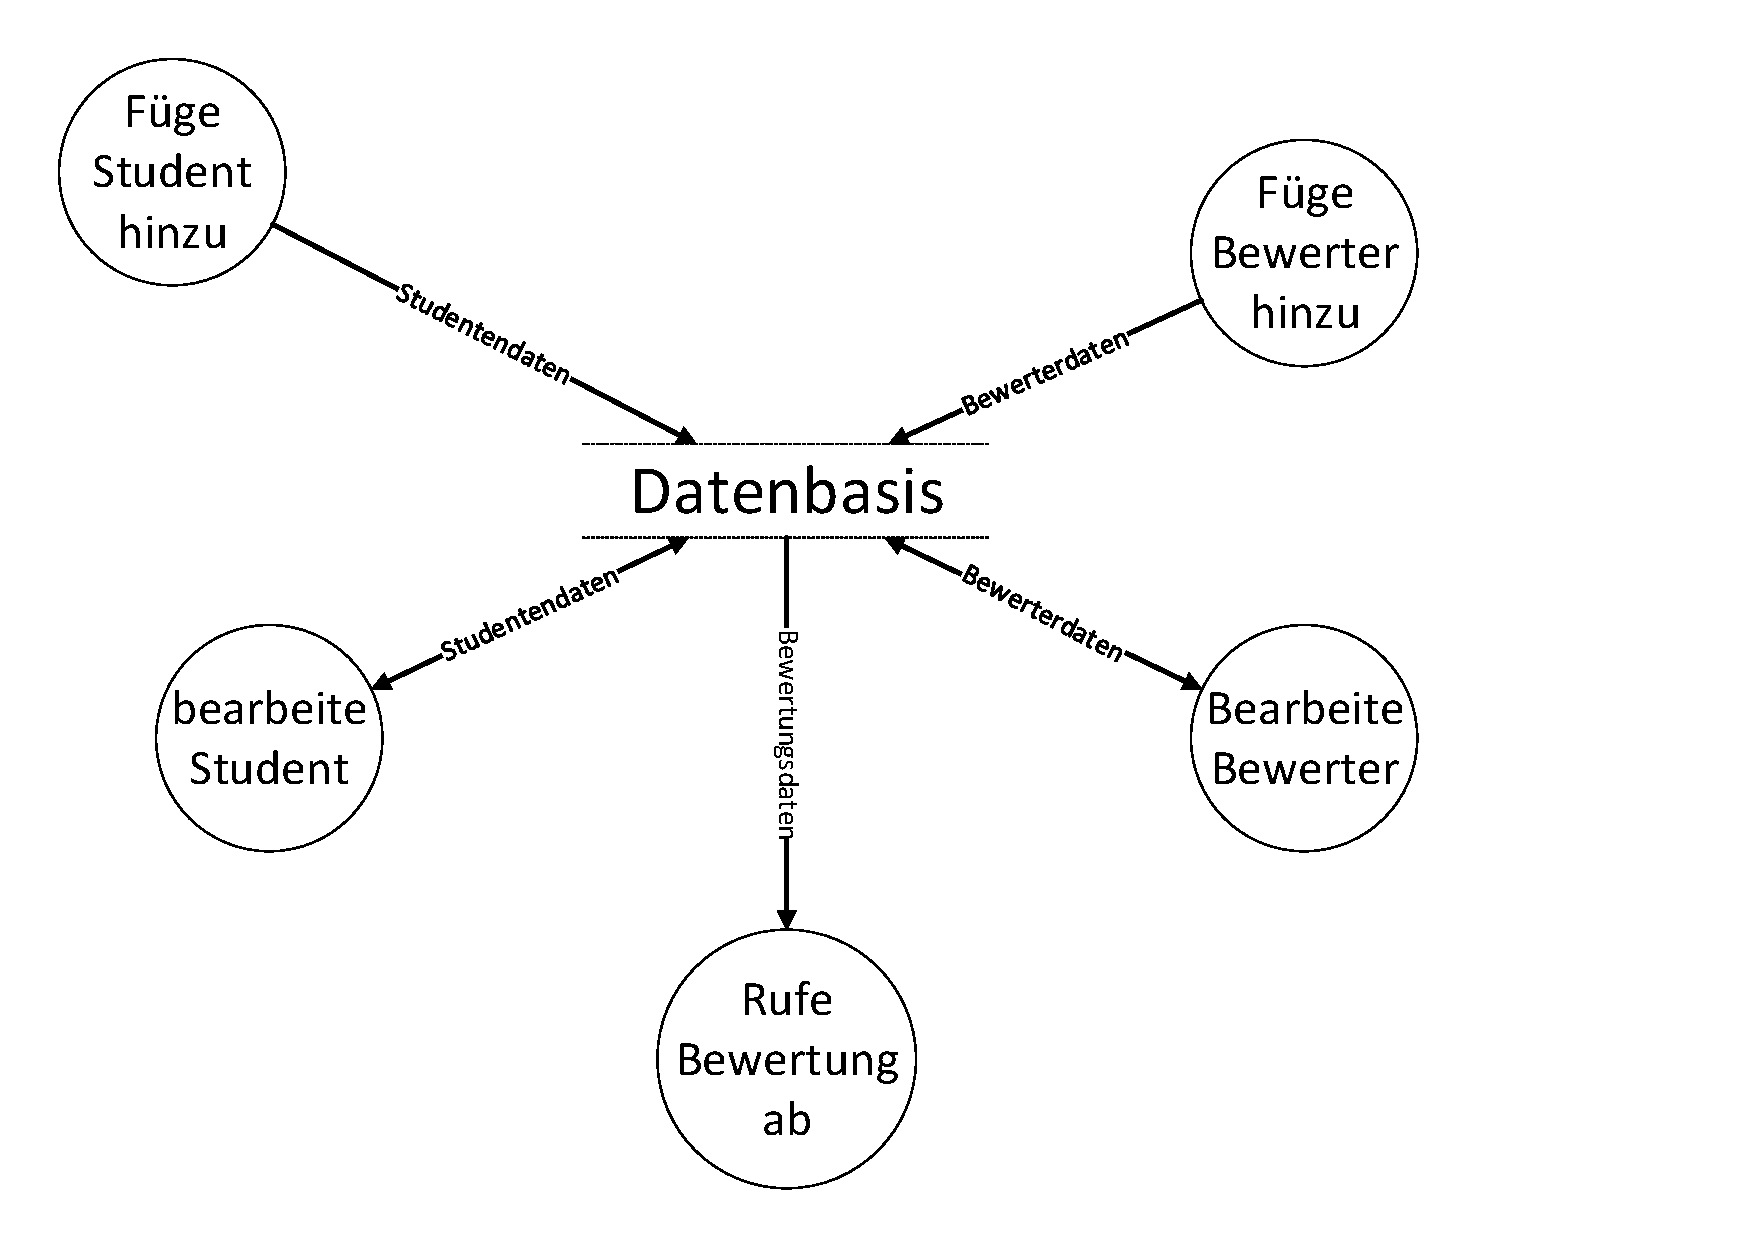
\includegraphics[width=1.4\textwidth, angle=90, origin=c]{../Diagramme/Kontextdiagramm_DFD2_Verwalter.pdf}
		\caption{Datenflussdiagramm Student}
	\end{figure}
	
	
	\listoftables
		
\end{document}